\documentclass[11pt,a4paper]{article}
\usepackage[latin1]{inputenc}
\usepackage{amsmath}
\usepackage{amsfonts}
\usepackage{mathtools}
\usepackage{array}
\usepackage{pifont}
\usepackage{ifsym}
\usepackage{booktabs}
\usepackage{listings}
\usepackage{amssymb}
\usepackage{graphicx}
\usepackage{longtable}
\usepackage{tabularx}
\usepackage{enumitem}
\usepackage{url}
\usepackage[margin=0.8in]{geometry}
\usepackage[toc,page]{appendix}
\usepackage{etoolbox}
\usepackage{morefloats}
\usepackage{multirow}
\usepackage[hidelinks]{hyperref}
\usepackage{float} % Allows putting an [H] in \begin{figure} to specify the exact location of the figure
\usepackage{verbatim}
\usepackage{listings}

\usepackage{fullpage}

\graphicspath{{img/}}

\patchcmd{\thebibliography}{\section*}{\subsection}{}{}

% Table padding
\renewcommand{\arraystretch}{1.5}

\begin{document}

\begin{titlepage}

\begin{center}

\includegraphics[width=0.5\textwidth]{img/University_Logo}\\

\textsc{\LARGE Swansea University }\\[0.5cm]
\textsc{\large MEng Computing }\\[2cm]

{ \huge \bfseries Group Project CS-M04}\\[0.2cm]
\textsc{\large Team Structure, Methodology, Requirements and Specifications}\\[1.5cm]

\begin{minipage}{0.4\textwidth}
\begin{flushleft}

\emph{Authors:}\\
Adam \textsc{Barrell} {\scriptsize \emph{(632975)}} \\
Thomas \textsc{Milner} {\scriptsize \emph{(637755)}} \\
Lewis \textsc{Hancock} {\scriptsize \emph{(xxxxxx)}} \\
Christopher \textsc{Lewis} {\scriptsize \emph{(xxxxxx)}} \\

\end{flushleft}
\end{minipage}
\begin{minipage}{0.4\textwidth}
\begin{flushright}

\emph{Supervisor:}\\
Parisa \textsc{Eslambolchilar}

\end{flushright}
\end{minipage}\\[1.3cm]

{\today}
\end{center}

\end{titlepage}

\newpage 

\tableofcontents

\newpage
\section{Introduction}
%- Purpose of Document (who it's for, outline Digital Trails briefly again).
%- Outline of Document (what we cover in the document).

\section{Technology Choices}
%- What APIs, Libraries, IDEs etc we are using, compared with other options we had. Argue our choices.

\subsection{The API}
To keep the Application and the website in sync, and allow for future developements such as aditional applications, an RESTful API (Application Programming Interface) was created.

\begin{description}
\item[API] Application Programming Interface, In general an API is a method of interaction between two software components through code. This often take the form of a Library, although a web API generally takes the form of several remote calls which are exposed to the user of the API. 

\item[REST] Representational State Transfer, is a architecture style which was used to design HTTP/1.1 (Hyper Text Transfer Protocol Version 1.1) and the URI (Universal Resource Identifier) standards. It consists of a set of constraints on components, data and there connections. The primary constraint is a Client-Sever separation, with the server being responsible for data storage, and the client responsible for the user interface and user state. The server is also required to be stateless which means no client context can be stored on the server.
\end{description}

For the API the Slim Framework\cite{slim} was chosen. This framework is designed for creating lightweight restful API's and websites and provides a versatile and well tested bases for the work. There were several other choises for this framework, but Slim was chosen becouse it was the most popular and well documented option. The Paris ORM(Object Relation Mapper) Framework\cite{paris} was also chosen to assist in database access. The ORM uses simple database models to reduce the steps in the process of interacting with the database. This framework makes it very easy to work with databases, drastically cutting the code needed to retrieve data and process it into objects. For example, if you had a simple database with just Documents and Users it would be possible to model this using just the code below. There are two model definitions and then 2 very basic lines of code which return a user object in the variable \lstinline{$user}. The second line then queries \lstinline{$user} to get all the documents associated with that user. \cite{TomMilestone2} 

\begin{lstlisting}
class User extends Model {
	public function documents(){
		return $this->has_many('Document');
	}
}

class Document extends Model{
	public function user(){
		return $this->belongs_to('User');
	}
}

$user = Model::factory('User')->find_one($id); 
$documents = $user->documents()->find_many();
\end{lstlisting}

\subsection{The Server}
The project is currently hosted on an Amazon EC2 server owned by a group member. Having a private server like this has allowed us to configure it as we require. The server is currently running Ubuntu Linux with Apache webserver, PHP and MySQL database installed. Git is used to push documents up to the server which are then automatically coppied into the correct folder for the webserver. Each part of the project can then be given a unique subdomain for testing purposes. Currently the API is hosted at \url{http://whiterockapi.tmilner.co.uk/} and the Web Portal is at \url{http://whiterock.tmilner.co.uk}.


\section{Project Progress}
%- THIS IS THE OVERVIEW SECTION
%- Show the subsystem designs and explain the current structure of the project. 
%- Possible to move the risk management and schedule sections up here if people feel it reads better. Depends how big those sections get.
%- Mention Amazon EC2 for testing purposes

\subsection{Database}

%- Why do we need a database, what data will it store?
A relational database has been created to store persistent data for the web portal and Android application.
The database stores data relating to entities such as walks, way points, users and media locations.
The database is currently hosted by an Amazon EC2 server (see technology choices) using MySQL.

%- How was the database designed?
The database schema was designed using Visual Studio's entity designer which allows developers visually develop databases.
This tool allows tables to be created on a canvas where relationships and attributes can be modified.
A table was created for each entity or concept that required persistent storage as shown in Figure \ref{fig:DatabaseSchema}.
Columns were then added to each table to represent the attributes of each entity.
For example, the \emph{EnglishWalkDescription} table has an \emph{Id}, \emph{Title}, \emph{ShortDescription} and \emph{LongDescription}. The column \emph{Id} is mandatory for standalone entities as the rest of their properties are identified by this unique key. 

%- How was the database be generated from this model?
The Visual Studio entity designer was able to generate an SQL script to create the database from the design shown in Figure \ref{fig:DatabaseSchema}. This script was executed on the MySQL server which in turn created the tables designed in the entity designer.

%- How will the database be exposed if not directly?
The White Rock Trails database is not publicly exposed and can only be interfaced through a public facing API (see section XXXXX). 
This will ensure the robustness of the database as additional business logic from the API protects the underlying database from erroneous data and unauthorized access.

%- What applications will consume data from this database?
The web portal and Android application will both consume data from this database through the public API. 
The web portal will consume data with every request made by users from their web browser. 
In contrast, the Android application will synchronise a local copy of the database through the API. 
This ensures that the application can be used offline as many walks will not be in range of an internet access point.

%- How does it's design conform to the requirements?
The database design conforms to the requirements required by the client which are defined in the Initial Document. 
More specifically, the design shown in Figure \ref{fig:DatabaseSchema} is based on the initial schema design provided by the client. 
The initial schema contained tables that did not have a high normal form. 
English and Welsh translations were present in the same tables for both the walk and way point descriptions. 
These tables were normalised as shown in Figure \ref{fig:DatabaseSchema} by moving the English and Welsh descriptions into separate tables.
In addition, the media locations for each way point were also present in the same table.
This was normalised by moving different media types such as images, audio and video into tables \emph{WaypointImage}, \emph{WaypointAudio} and \emph{WaypointVideo} respectively.

%- Describe the relationships (one-one) (one-many) (many-many)
Relationships were defined between tables using Visual Studio's entity designer. 
The designer supports a range of associativities such as one-one (1-1), one-many (1-*) and many-many (*-*). 
Some of these associativities were used in the White Rock Trails schema as shown in Figure \ref{fig:DatabaseSchema}.
For example, the \emph{Walk} entity can have many \emph{WalkReviews}, one \emph{User} who created it, many \emph{Waypoints}, one \emph{EnglishWalkDescription} and one \emph{WelshWalkDescription}.

\begin{figure}[h!]
\centering
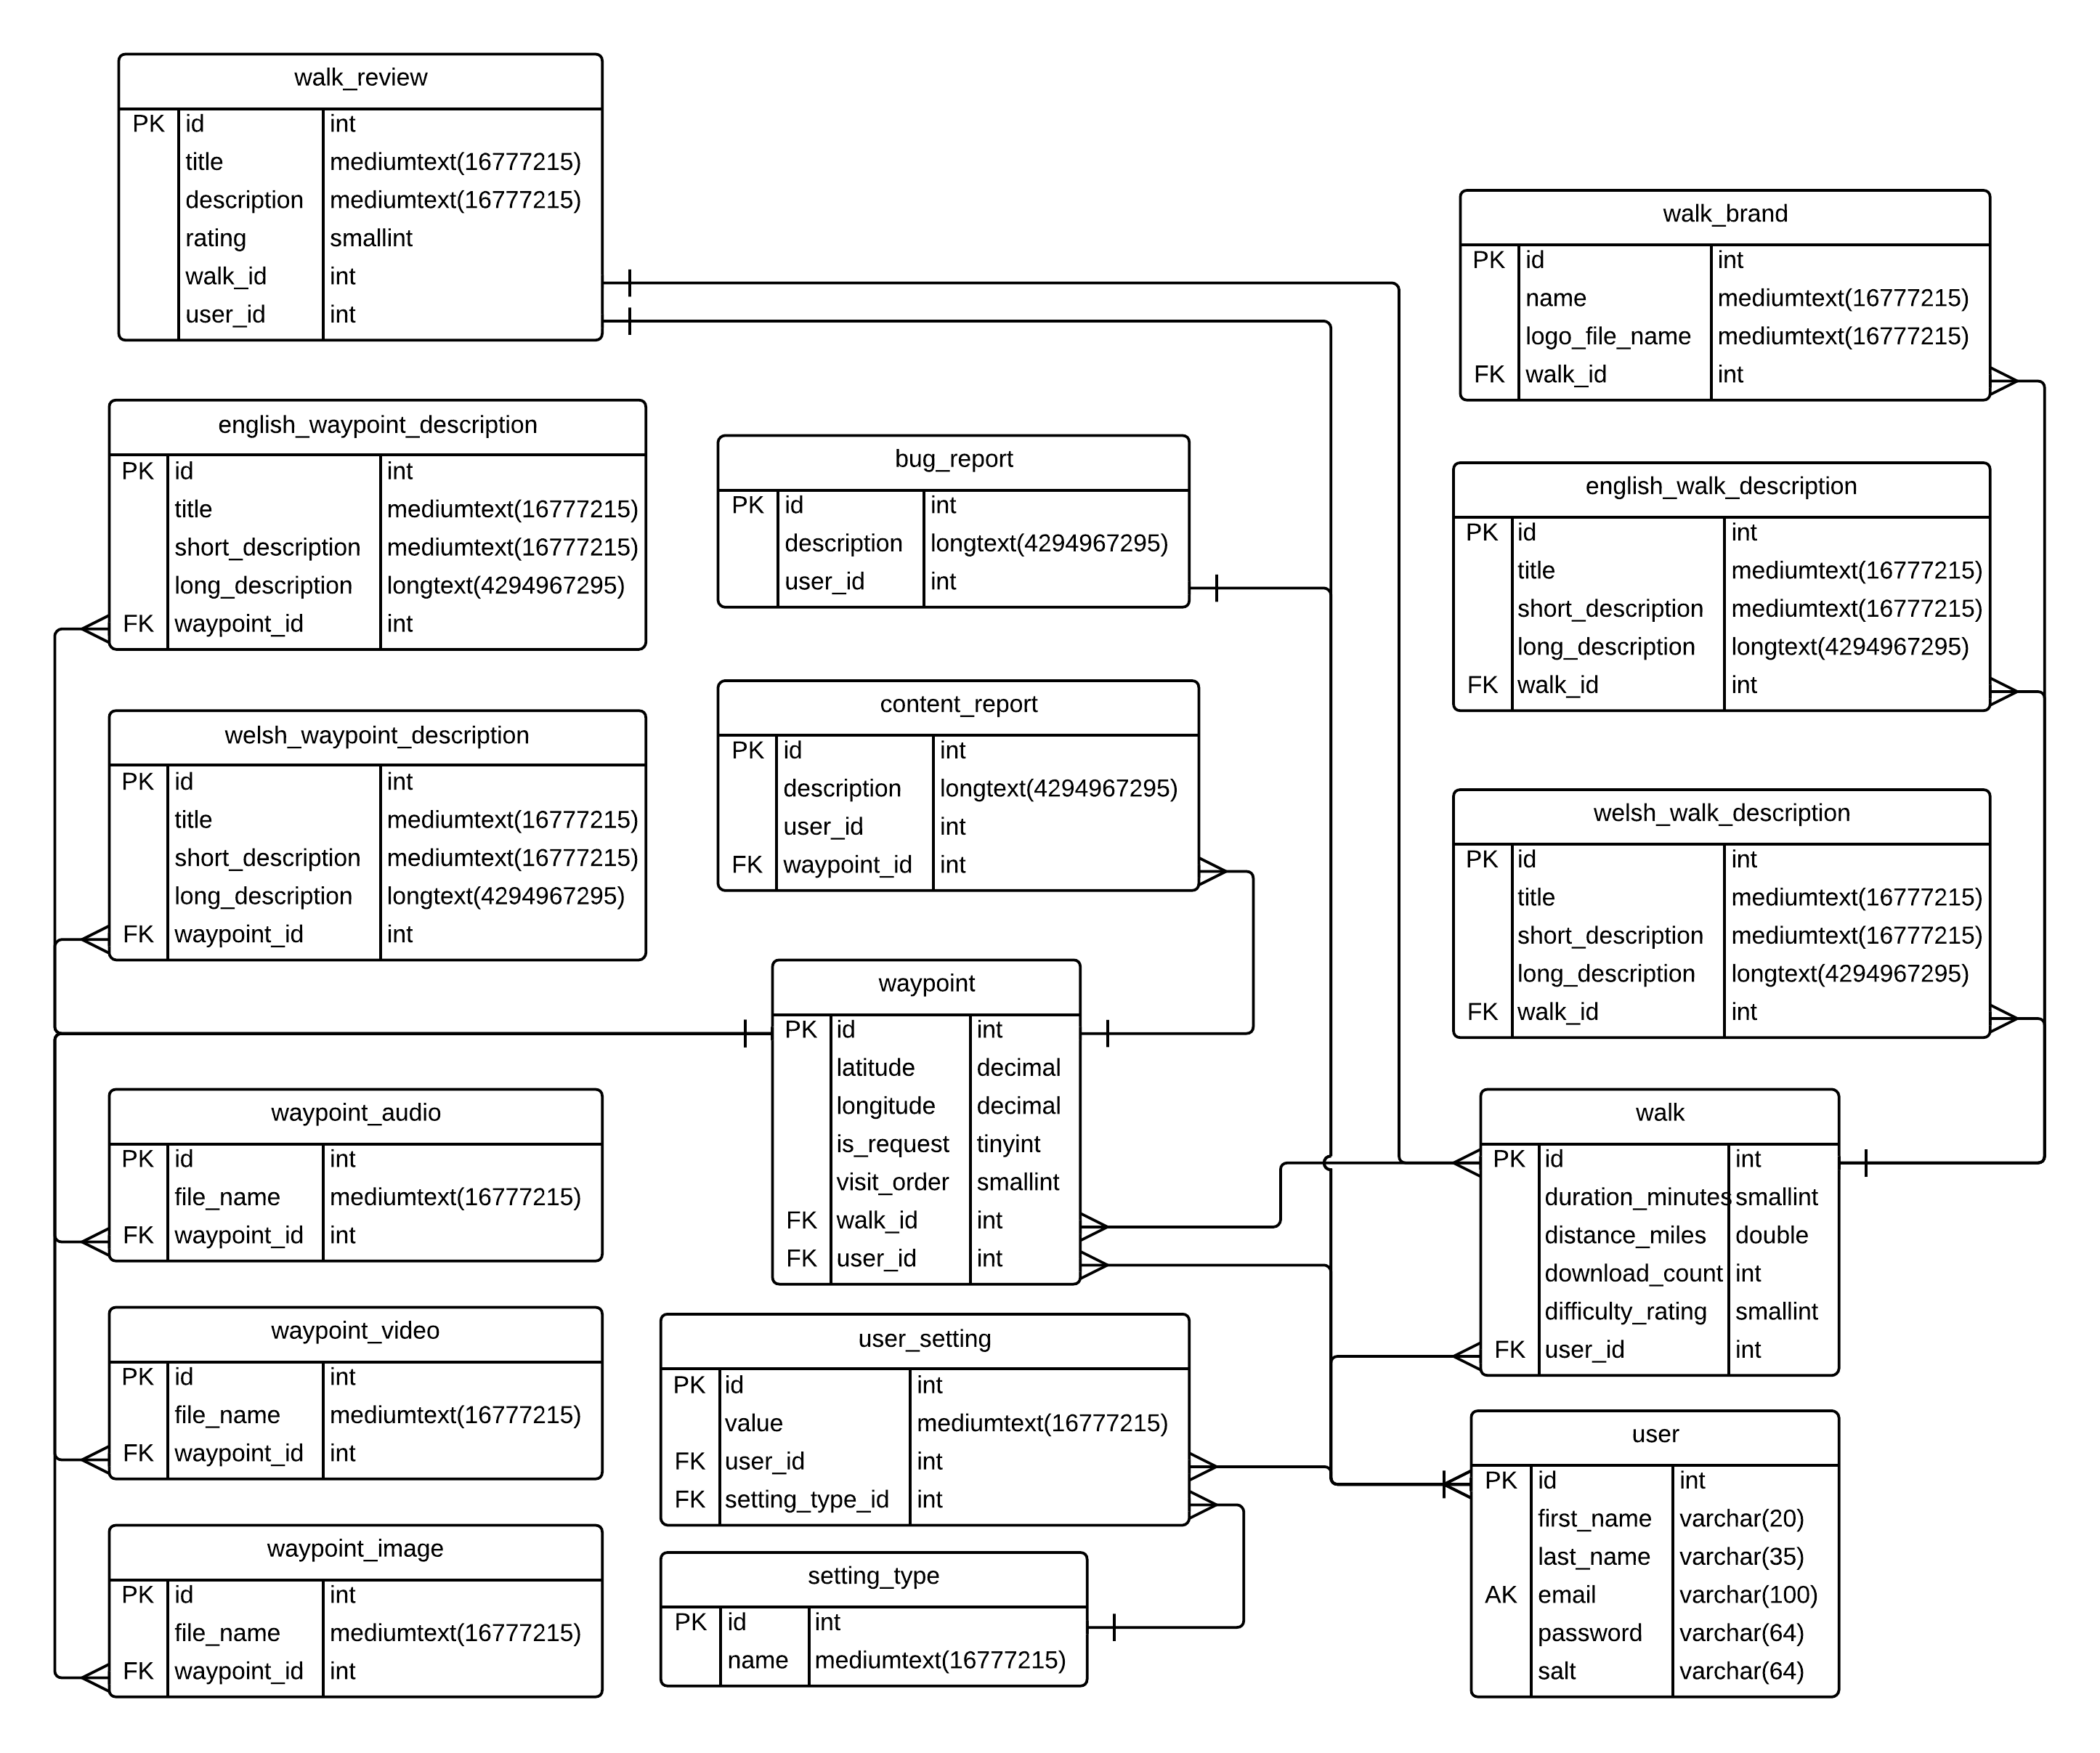
\includegraphics[angle=90, width=1\linewidth]{./img/DatabaseSchema}
\caption{Schema of the White Rock Trails relational database.}
\label{fig:DatabaseSchema}
\end{figure}


\subsection{User Interfaces}
%- Heuristic Evaluations on similar products
%-- Explain how we are doing the evaluation blahblah nielsen etc.
%-- List of tasks for evaluators to complete (we should really ALL be involved in doing the evaluations).
%-- Problems found when completing each task
%- Our prototype UI 1
%-- show how it meets reqs, how heuristics helped design.
%-- Heuristics on this etc.
%- Our prototype UI 2
%-- show it meets reqs, how heuristics helped design.
%-- Heuristics
%- repeat as necessary.

\subsection{Android Application}
%- ContentProvider
%- Authorisation
%- Google Maps
%- Current design to sync with server
%- Chris can chuck in his Fragments here, so he has some code to show.


\subsection{API}

There are several important parts to the API, first it must have a coherent set of routes/urls for acces to all if its functionality, secondly it must provide a method of authenticating users and finaly it must adhear to to principles of REST as closely as possible. 

\subsubsection{Routes}

The API is called through a series of routes, it was important to make these routes as simple and coherant as possible.

\begin{longtable}{p{0.45\textwidth}|p{0.35\textwidth}|p{0.1\textwidth}}\hline
    \textbf{Route} & \textbf{Return value} & \textbf{Methods} \\\hline
    /walks & All walks & GET, POST\\ \hline
    /walks/\$id & The walks with the ID \$id. & GET PUT DELETE\\ \hline
    /walks/\$id/waypoints & All the waypoints for the walk with the ID \$id. & GET POST\\ \hline
    /walks/\$id/waypoints/\$wid & The waypoint with the ID \$wid. & GET PUT DELETE \\ \hline
    /walks/\$id/waypoints/\$wid/images & The images for the waypoint with the ID \$wid. & GET POST \\ \hline
    /walks/\$id/waypoints/\$wid/images/\$iid & The image with the ID \$iid. & GET PUT DELETE \\ \hline
    /walks/\$id/waypoints/\$wid/audio & The audio files for the waypoint with the ID \$wid. & GET POST \\ \hline
    /walks/\$id/waypoints/\$wid/audio/\$aid & The audio file with the ID \$aid. & GET PUT DELETE \\ \hline
    /walks/\$id/waypoints/\$wid/videos & The videos for the waypoint with the ID \$wid. & GET POST \\ \hline
    /walks/\$id/waypoints/\$wid/videos/\$vid & The video with the ID \$vid. & GET PUT DELETE \\ \hline
    /users & All users. & GET POST \\\hline
    /users/\$id & The user with the ID \$id. & GET PUT DELETE \\\hline
    /session & A request to authenticate. & GET\\\hline
    /session/salt & Returns a random salt for registering a user. & GET\\\hline
    /session/salt/\$username & Get the a salt for a specific user with the username \$username. & GET\\\hline
    \caption {The routes for the API}
    \label{routes}
\end{longtable}

\subsection{Web Portal}

%- What progress has been made on the web portal?
This section discusses the progress which has been towards development of the web portal. The web portal will allow users of the Android application, full control over the management of their walks. This includes the addition and modification of walks, contributions to other user's walks and the attachment of media such as video, images and audio to specific way points. The web portal aims to provide users with a more intuitive interface to manage walks since the modification of data can be difficult through mobile devices with small screens. 

%- Currently what does the portal allow users to do?
A number of features have been developed thus far, including login, registration, responsive layouts, form validation and walk views. Figure \ref{fig:home} shows the first web pages that users will be greeted with upon visiting the web portal. As shown in the diagram, the web portal features distinct White Rock Trails branding which has been designed specifically for this project. This is also a requirement of the software as requested by the client. The visual theme and layout of the web portal has been designed to imitate that of the Android application. This will make the web portal more intuitive to users and its learning curve will be significantly reduced.

%- What tools have been used to create it?
An IDE (Integrated Development Environment) called Brackets was used to develop the web portal. This software features automatic code completion for JavaScript and GIT integration. The former greatly enhanced development productivity while the latter allowed for easy code collaboration between the programming team. The web portal is currently hosted on a public Amazon EC2 server. This allows the client to interact with the latest web portal version and suggested improvements or alterations.

\subsubsection{Welcome View}

The welcome view shown in Figure \ref{fig:home} provides visitors with a link to download the Android application and instructs them to login or register account in order to use the portal. A footer has also been added to provide users with navigation links to important resources such as the Android application and \emph{About} page.

\begin{figure}[h!]
\centering
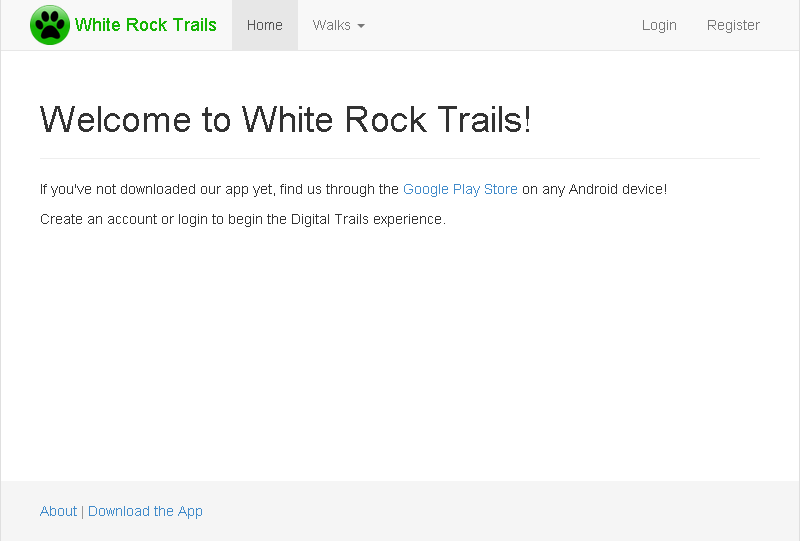
\includegraphics[width=0.8\linewidth]{./img/webportal/home}
\caption{Home view of the web portal.}
\label{fig:home}
\end{figure}

\subsubsection{Responsive View}

Figure \ref{fig:home-responsive} demonstrates a responsive review of the web portal. This is the view that users will see when visiting the web portal on mobile devices such as smart phones and tablets. The responsive design minimizes the menu bar which can be expanded by clicking the button shown in the top right of the figure. In addition, web page content reduces in width and elements become stacked allowing for easier scrolling on mobile devices. The responsive design of the web portal is facilitated by the Bootstrap (see section XXXXXX) CSS and JavaScript library.

\begin{figure}[h!]
\centering
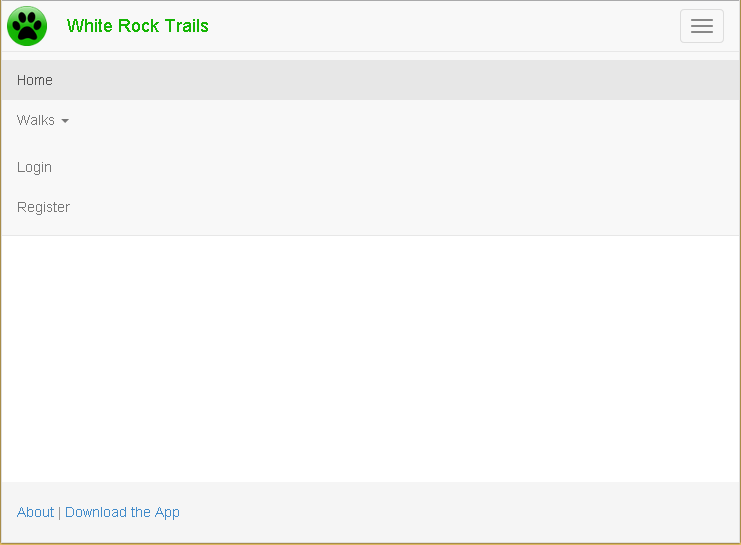
\includegraphics[width=0.8\linewidth]{./img/webportal/home-responsive}
\caption{Web portal responsive menu view.}
\label{fig:home-responsive}
\end{figure}

\subsubsection{Login View}

Figure \ref{fig:login} shows the login view that users will see when they click on the \emph{Login} button in the top navigation bar. The login view displays as a modal in front of the web page. This will ensure that users do not have to navigate between pages in order to log in, thus enhancing usability. The login view requires users to input their email address and password followed by clicking the \emph{Login} button. The \emph{Login} button will display a spinner icon whilst the fields are validated to ensure the user is aware that the page is loading. An external validation library is used to validate the fields and display an error or success status. The library uses pre-defined validators to validate the structure of the email address and that the email and password pair is valid when checked against the White Rock Trails API. The validator changes the display of erroneous fields to feature red or green borders and tick or cross icons for invalid and valid fields respectively. A specific error message will also be displayed underneath erroneous fields to inform the reason for the error and allow users to amend it. When users successfully log in, the modal will close and the \emph{Login} and \emph{Registration} buttons shown in the top navigation bar are replaced with the user's full name.

\begin{figure}[h!]
\centering
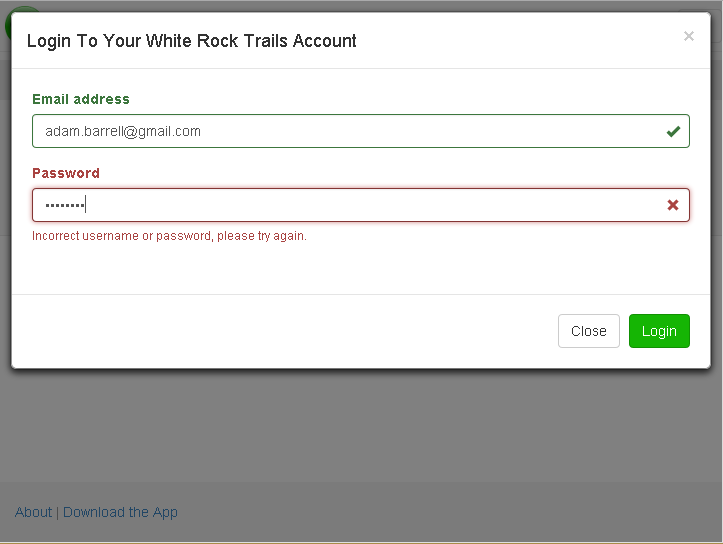
\includegraphics[width=0.8\linewidth]{./img/webportal/login}
\caption{Web portal login modal demonstrating validation.}
\label{fig:login}
\end{figure}

\subsubsection{Registration View}

Figure \ref{fig:registration} shows the registration view that users will see when the \emph{Register} button is clicked in the top navigation bar. This view is also implemented as a modal for the same reasons as the login view and to maintain consistency throughout the application. The same validator is also used to validate the registration fields. However, inputs such as \emph{Email Address} and the two password fields require different validators. The former uses a validator that checks whether the provided email address has already been registered by another user. The latter checks whether the two passwords are identical. This will prevent users from registering using a mistyped password and subsequently not being able to log in. Clicking the \emph{Register} button will display a loading spinner inside as described for the login view. When users successfully register, they will be presented with a new confirmation modal instructing them to log in with their new account.

\begin{figure}[h!]
\centering
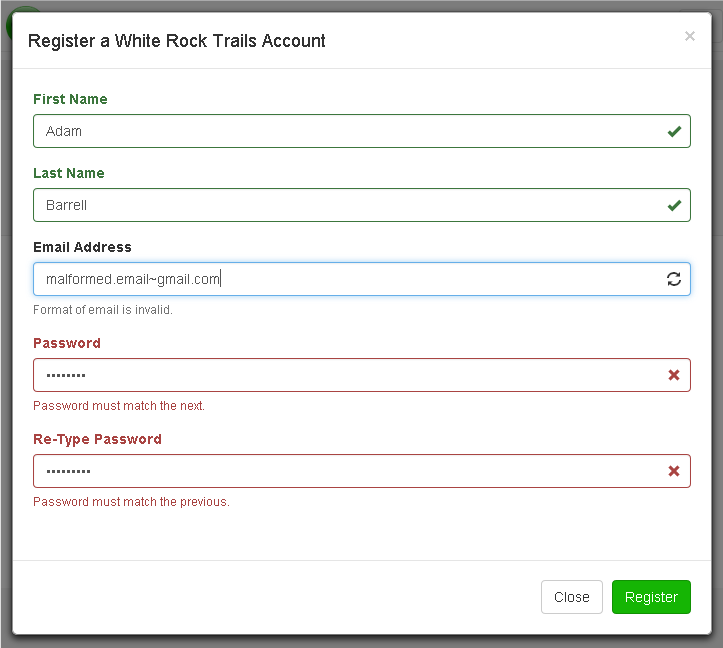
\includegraphics[width=0.8\linewidth]{./img/webportal/registration}
\caption{Web portal registration modal demonstrating validation.}
\label{fig:registration}
\end{figure}

\subsubsection{All Walks View}

Figure \ref{fig:all-walks} shows the view users will see when they click on the \emph{Walks} button in the top menu bar and select the \emph{All Walks} option. This view displays a list of tiles, each representing a walk in the database. The background of each tile is an image selected from the collection of each walks way point images. Clicking a tile will navigate the user to a walk information view as presented in Figure \ref{fig:walk-info}. The \emph{Add Walk} button and search bar are currently non-functional as those features have not yet been implemented.

\begin{figure}[h!]
\centering
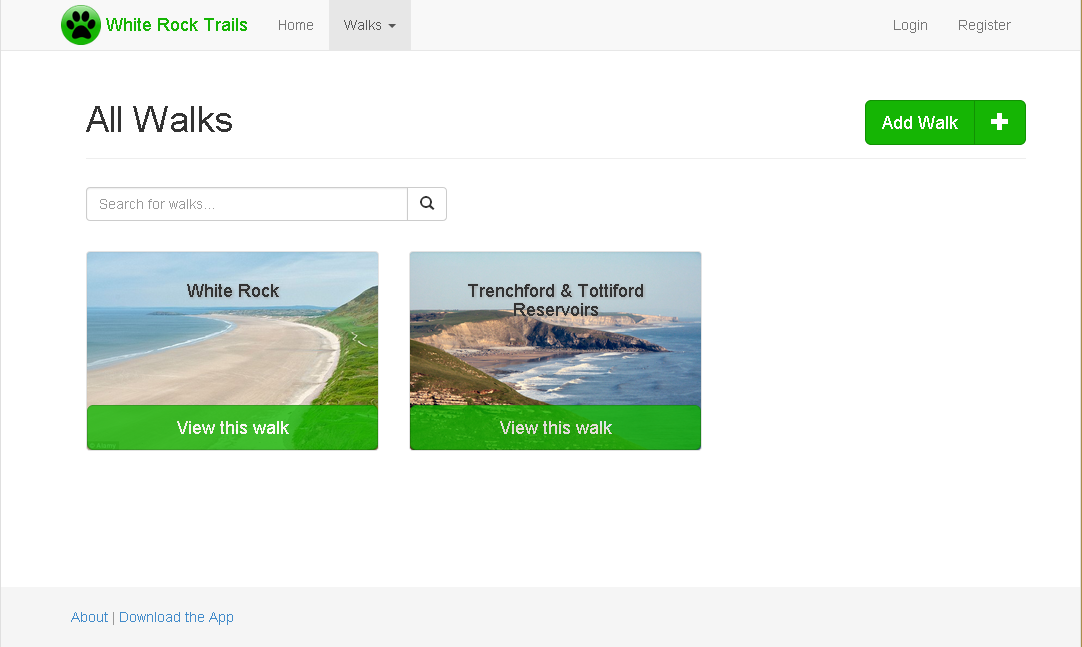
\includegraphics[width=0.8\linewidth]{./img/webportal/all-walks}
\caption{All walks view of the web portal.}
\label{fig:all-walks}
\end{figure}

\subsubsection{Walk Information View}

Figure \ref{fig:walk-info} shows the view users will see when they click on a walk tile from the \emph{All Walks} view. As shown in the figure, walk information will be displayed in this view such a title, description, duration, distance, difficulty rating and author. Navigation tabs above this information allow users to navigate between the \emph{Waypoints}, \emph{Reviews} and \emph{Walk} views. Walk data is asynchronously loaded from the database through the API. The Google Maps API is used to display the map shown in the right of the figure. The Google Maps API allows markers to be placed at specific GPS locations contained within the walk data. The map allows users to scroll and zoom around the walk area to gain an understanding of its location.

\begin{figure}[h!]
\centering
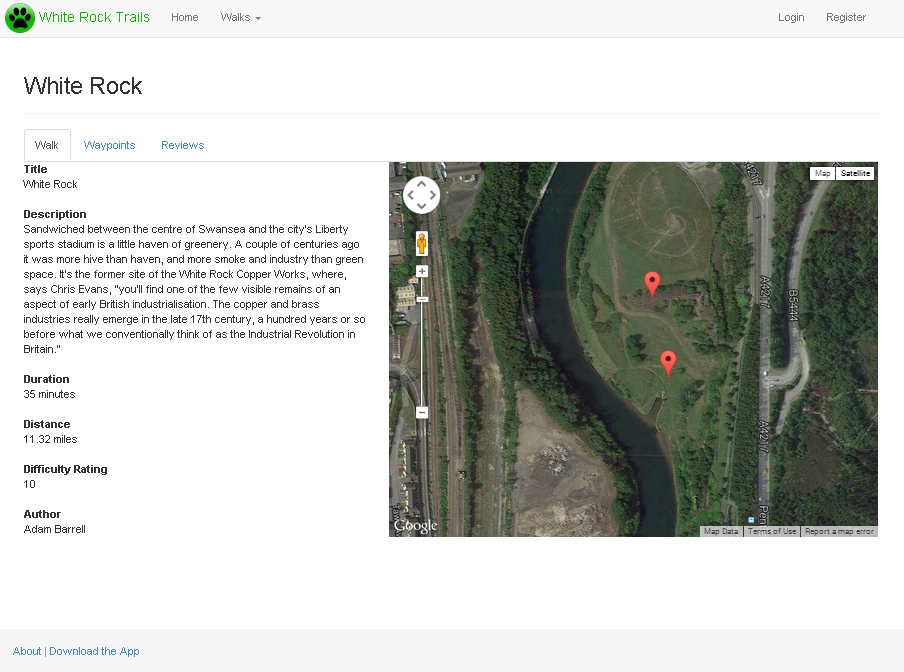
\includegraphics[width=0.8\linewidth]{./img/webportal/walk-info}
\caption{Walk information view of the web portal.}
\label{fig:walk-info}
\end{figure}

\subsubsection{Walk Way Points View}

Figure \ref{fig:walk-waypoints} shows the view that users will see when they click on the \emph{Waypoints} tab of the walk information view. The view shows the list of way points that are represented by markers on the map. Clicking a list item or its corresponding map marker will display a modal containing media uploaded to the way point such as images, videos and audio. However, this feature is still in progress and is not shown in this document.

\begin{figure}[h!]
\centering
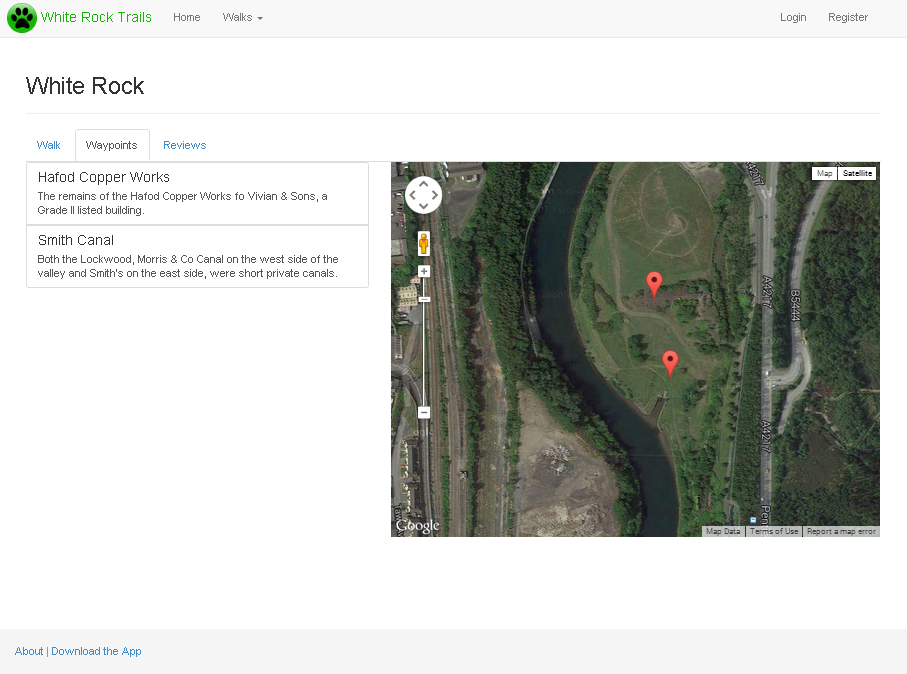
\includegraphics[width=0.8\linewidth]{./img/webportal/walk-waypoints}
\caption{Walk way points view of the web portal.}
\label{fig:walk-waypoints}
\end{figure}

\subsubsection{Walk Reviews View}

Figure \ref{fig:walk-reviews} shows the view that users will see when they click the \emph{Reviews} tab from the navigation tabs bar. This view loads user reviews from the walk data and displays them in a list view as shown in the figure. A library called \emph{Raty} was used to generate the star rating system seen below the title of the review. It takes a review rating integer between 1-5 and generates a star representation.

\begin{figure}[h!]
\centering
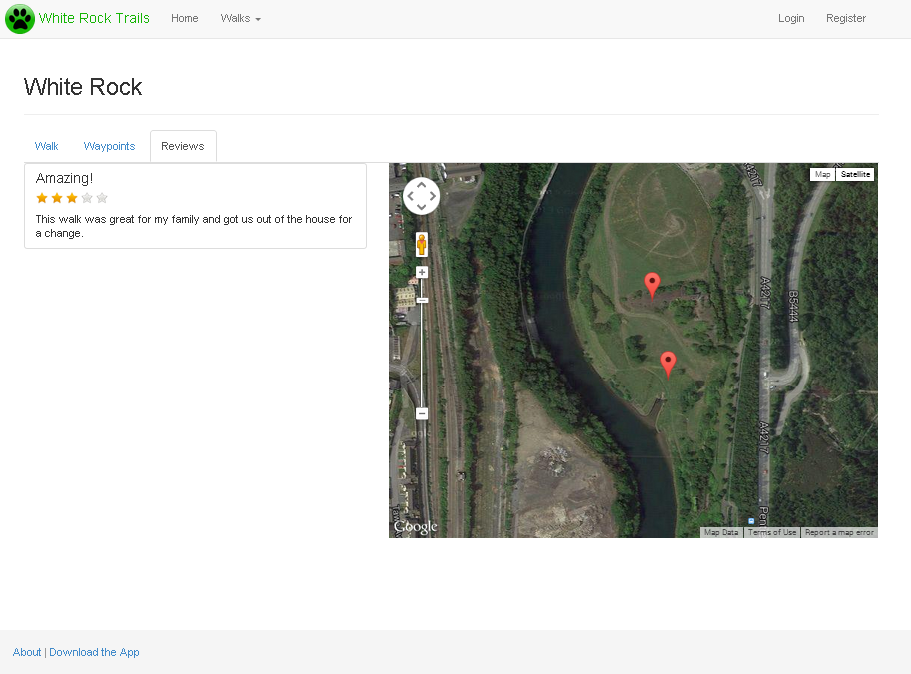
\includegraphics[width=0.8\linewidth]{./img/webportal/walk-reviews}
\caption{Walk reviews view of the web portal.}
\label{fig:walk-reviews}
\end{figure}


\section{Programming Guidelines}
%- I'll write android guidelines.
%- Adam/Tom get on the web guidelines.

\section{Risk Analysis Review}
%- Explain risks we dealt with, cross reference to our initial table.
%- Add new risks that arose (Poor work environment, lab computers suck, hudl broken, hudl missing USB driver - not supported as a dev. device).

\section{Project Schedule Review}
%- What sprints we have completed.
%- What reqs / specifications are completed Chris Lewis' favourite job!).
%- Are we ahead or behind schedule? (hard for us to answer)
%- Did we have to modify any requirements / specs to get this far? Did we add any or drop any?
%- Create new gantt chart and compare it with the initial one.
%- Update online sprint software, make it look like we completed sprints on time.
%- Client feedback so far, previous client meetings, planned meetings, launch event we attended etc.

\section{Summary}
%- What we have planned next, I guess.

%References as subsection
\newpage
\bibliographystyle{plain}
\bibliography{bibliography}
\end{document}